% !TEX encoding = UTF-8 Unicode
\chapter{Umsetzung}
In diesem Kapitel wird beschrieben, wie Esper installiert werden kann. Die in der Implementierung entwickelte Java-Anwendung, verwendet Esper im Kontext des Szenarios (siehe Kapitel \ref{Szenario}) dieser Arbeit.
\section{Installation}
Für die Installation von Esper wird in dieser Ausarbeitung des Build-Tool \textbf{Apache Maven} verwendet. 
Dieses ermöglicht das automatisierte Herunterladen der Esper-Engine. Hierzu wird eine Konfigurationsdatei für Maven benötigt, die sogenannte \textbf{pom.xml}. Nachfolgend wird diese für das Szenario dargestellt:

\begin{lstlisting}[caption={Maven-Konfiguration}\label{lst:mavenKonfiguration},captionpos=t,language=XML]

<?xml version="1.0" encoding="UTF-8"?>
    <project xmlns="http://maven.apache.org/POM/4.0.0"
     xmlns:xsi="http://www.w3.org/2001/XMLSchema-instance"
     xsi:schemaLocation="http://maven.apache.org/POM/4.0.0
     http://maven.apache.org/xsd/maven-4.0.0.xsd">
		
     <modelVersion>4.0.0</modelVersion>

     <groupId>de.htwg.da</groupId>
     <artifactId>esper-sample</artifactId>
     <version>1.0-SNAPSHOT</version>

     <dependencies>
         <dependency>
             <groupId>com.espertech</groupId>
             <artifactId>esper</artifactId>
             <version>7.1.0</version>
         </dependency>
     </dependencies>
</project>
\end{lstlisting}

Wichtig ist hierbei das XML-Element \textbf{<dependencies>} welche die Abhängigkeiten enthält. Diese werden automatisch heruntergeladen, sobald Maven ausgeführt wird. In der Beispiel-Konfiguration gibt es nur eine Abhängigkeit, die für Esper.

Nach dem Download kann die Esper-Engine direkt bei der Entwicklung einer Java-Anwendung verwendet werden. Für andere Sprachen, sind unter Umständen Build-Tools zu verwenden, welche hier nicht beschrieben werden.

\section{Implementierung}
Dieses Kapitel beinhaltet die einzelnen Schritte der Implementierung des Szenarios (beschrieben in Kapitel \ref{Szenario}). Zu beginn werden die erzeugten Event-Klassen beschrieben, anschließend wird das Versenden der Events und deren Verarbeitung behandelt.
\subsection{Event-Klassen}
\begin{figure}[ht]
	\centering
	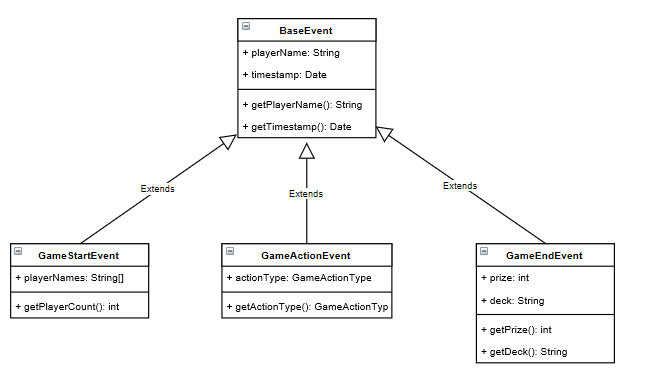
\includegraphics[width=\textwidth,height=\textheight,keepaspectratio]{images/Events.png}
	\caption{Event Klassen des Szenarios}
	\label{EventKlassen}
\end{figure}
Um das Szenario abzubilden werden verschiedene Event-Klassen benötigt. Mit diesem Begriff sind Klassen gemeint, die ein Event darstellen.
Als gemeinsame Basis dient die Event-Klasse \textbf{BaseEvent} (Siehe Abbildung \ref{EventKlassen}). Dieses Event beinhaltet den Spieler-Namen und einen Zeitstempel. Diese beiden Felder werden in allen Events benötigt.

Die Event-Klassen \textbf{GameStartEvent} und \textbf{GameEndEvent} bilden den Start und das Ende einer Poker-Partie ab. Zu Beginn (GameStartEvent) werden alle Spiel-Teilnehmer benötigt, gegen Ende (GameEndEvent) das Preisgeld und Kartendeck, welches gewonnen hat. Da beide Events von \textbf{BaseEvent} erben, besitzen sie automatisch einen Zeitstempel und den zugeordneten Spieler. Beim Spielstart wird der Name des ersten Spielers verwendet.

Im Laufe der Partie werden verschiedene Aktionen der Spieler durchgeführt. Diese sind durch die Event-Klasse \textbf{GameActionEvent} abgebildet. Das Event beinhaltet ein Feld für die Aktionsart (z.B. "rise", wenn ein Spieler erhöht hat).

\subsection{Events versenden}
Für das Versenden eines Events wird die Methode \textbf{sendEvent(...)} der Klasse \textbf{EPRuntime} verwendet (siehe Architektur, in Kapitel \ref{architektur}). Als Parameter kann eine beliebige Event-Klasse übergeben werden, wie nachfolgend mit einem \textbf{GameStartEvent} dargestellt:
\begin{lstlisting}[caption={Event versenden}\label{lst:fireEvent},captionpos=t,language=Java]

EPServiceProvider cep = EPServiceProviderManager.
			getProvider("MyEsperProvider",esperConfig);

final EPRuntime cepRT = cep.getEPRuntime();

// Fire sample event
cepRT.sendEvent(new GameStartEvent());
\end{lstlisting}
Damit die Events für das Szenario einfach erzeugt und versendet werden können, wird eine Generator-Klasse verwendet, im Folgenden \textbf{EventGenerator} genannt. Darunter versteht man eine Klasse, die für das Generieren von Beispielwerten verwendet wird.

\begin{lstlisting}[caption={Event Generator}\label{lst:eventGenerator},captionpos=t,language=Java]
public final class EventGenerator {
  private static String[] PLAYER_NAMES = {"Clemens", "Lukas", "Kathrin"};
  private static Random GENERATOR = new Random();
  
  public static GameActionEvent randomGameActionEvent() {
    final String playerName = randomPlayerName();
    final Date timestamp = randomTimestamp();
    final GameActionType gameActionType = randomGameActionType();
    return new GameActionEvent(playerName, timestamp, gameActionType);
  }
	
  public static GameEndEvent randomGameEndEvent() {
    final String playerName = randomPlayerName();
    final Date timestamp = randomTimestamp();
    final int prize = GENERATOR.nextInt(500000);
    final Deck deck = randomDeck();

    return new GameEndEvent(playerName, timestamp, prize, deck);
  }

  public static GameStartEvent randomGameStartEvent() {
    final Date timestamp = randomTimestamp();

    return new GameStartEvent(PLAYER_NAMES, timestamp);
  }
	
  private static Deck randomDeck() {
    int deckIndex = GENERATOR.nextInt(Deck.values().length);
    return Deck.values()[deckIndex];
  }

  private static GameActionType randomGameActionType() {
    int gameActionTypeIndex = GENERATOR.nextInt(GameActionType.values().length);
    return GameActionType.values()[gameActionTypeIndex];
  }

  private static String randomPlayerName() {
    int playerIndex = GENERATOR.nextInt(PLAYER_NAMES.length);
    String playerName = PLAYER_NAMES[playerIndex];
    return playerName;
  }

  private static Date randomTimestamp() {
    long timeStamp = System.currentTimeMillis();
    return new Date(timeStamp);
  }
}
\end{lstlisting}
\subsection{Events verarbeiten}